% This is HBBNC and HBC
\label{section:HBBNC}
\label{section:HBC}
%\section{Abstract}
\section{Abstract}
In the following the samples are prepared with increasing surface coverage of HBBNC adsorbed at RT on Ag(111) and investigated by means of STM, AFM and XPS on Ag(111). The assemblies formed upon adsorption are studied and a binding motif for sub-ML coverage is derived. After annealing the regular assembly patterns are lost and a new binding motif is observed and investigated with STM and AFM. The molecules change their adsorption behavior on Au(111) where they separate into monomers arranged in the herringbone reconstruction.

\section{Introduction}
Graphene, a carbon honeycomb lattice, has interesting aspects for applications in electronics, its band gap is often subject of interest, determining the opto-electronic properties. Different methods to tune both include placement of ad-atoms below the lattice (intercalation) and replacement of individual lattice atoms (doping). To control the defect density on the atomic level, the desired stoichiometry is determined by growing graphene from precusor molecules. These molecules form self-assembled islands, their stoichiometry beeing determined by the precursor design. Polyaromatic hydrocarbons are the prototype of precursor material for graphene growth. 

Coronene ($C_{24}H_{12}$, known as [6]circulene or super benzene) is a polycyclic aromatic hydrocarbon made of six carbon rings to form a molecule reminiscent of a small graphene flake. It belongs to the family of circulenes where a central polygon is enclosed by different numbers of fused benzenoids. For example [5]circulene (corannulene), [6]circulene (coronene), [7]circulene and higher orders could be synthesized and show different conformation. While species with 5 or 7 benzene rings are bowl shaped, coronene is flat.

\section{The molecule}
\begin{figure}[ht]\centering
	\subfigure[HBC]{
		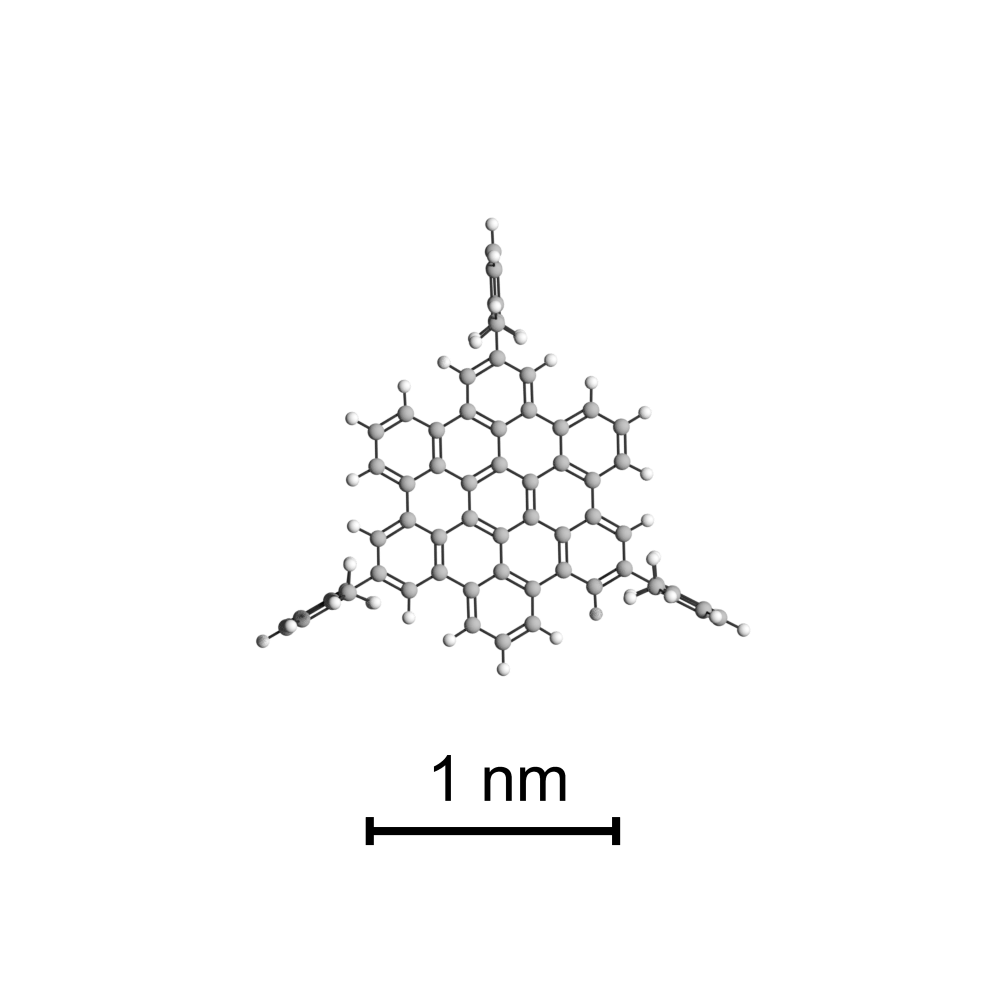
\includegraphics[width=0.45\textwidth]{./images/molecules/HBC-scalebar}
		\label{fig:HBC}
	} \quad
	\subfigure[HBBNC]{
		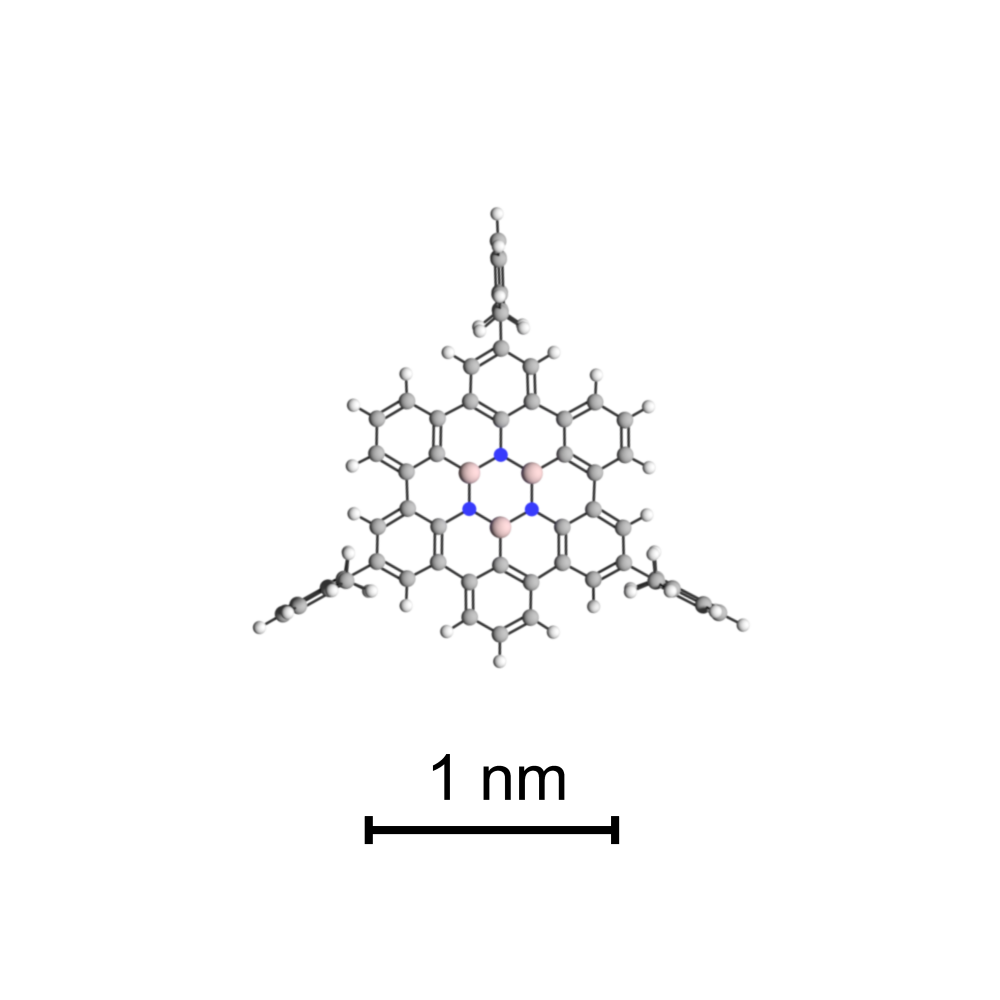
\includegraphics[width=0.45\textwidth]{./images/molecules/HBBNC-scalebar}
		\label{fig:HBBNC}
	}
	\caption{Geometric gas-phase calculated structure of \subref{fig:HBC} HBC and \subref{fig:HBBNC} HBBNC. While HBC is constituted solely of carbon, the central carbon ring in HBBNC is replaced with alternating boron and nitrogen atoms. Image width: \SI{4}{\nano \meter}}
	\label{fig:HBBNC+HBC}
\end{figure}

%\begin{wrapfigure}{R}{5cm}\centering
%	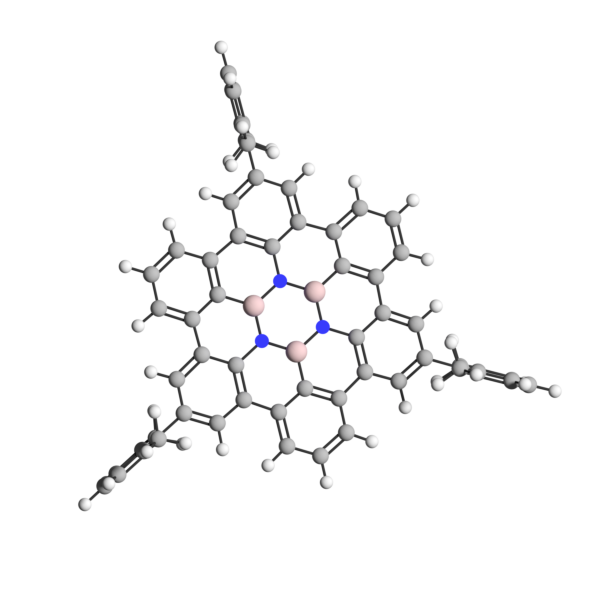
\includegraphics[angle=90,width=5cm]{./images/molecules/max-zoom/HBBNC-600}
%	\caption{HBBNC}
%	\label{fig:HBBNC-molecule}
%\end{wrapfigure}

Here we use modifications of coronene as shown in \autoref{fig:HBBNC+HBC}. For both species six benzene rings are added to extend the molecular backbone. Three 2,6-Dimethylphenyl groups were added to the molecules that now resemble a triangular footprint. While hexa‐peri‐hexabenzo-coronene (HBC shown in \autoref{fig:HBC}) features a central carbon ring, it is substituted by a central borazine ring for hexa‐peri‐hexabenzo-borazino-coronene (HBBNC shown in \autoref{fig:HBBNC}). Here the central $(BN)_3$ core is oriented to point all nitrogen atoms towards the leg functionalization. DFT calculations in gas-phase show a flat coronene center with upright standing legs for both species.

While in 2015 \cite{Krieg_construction_2015} and 2016 \cite{Ciccullo_Quasi-Free-Standing_2016} HBBNC was synthesized, its bad solubility prohibited experiments. In 2017 the synthesis \cite{dosso_synthesis_2017} of a soluble, BN-doped coronene derivative by substitution of the central carbon ring was successful. 

Both species have the same number of atoms and molecular weight. The difference between both becomes apparent when calculated electronic properties are compared (in gas phase). \autoref{fig:HBC+HBBNC-electronics} contrasts the electrostatic potential (ESP) and the band gap of the two species that have been done in the group of Prof.\ Dr.\ D.\ Bonifazi.\cite{dosso_synthesis_2017} The regular covalent $sp^2$ hybridization within the coronene core results in an evenly distributed electron density in HBC where the central region of the molecule shows considerable negative charge as a result of the molecules central $\pi-$system. Changing the central carbon ring to a borazine ring changes the ESP. Electrons are redistributed from the central borazine ring towards the outer hexaphenylene rim. In the center the aromaticity is interrupted and the extended electron $\pi-$system is altered because the ionic character in the bong between B and N. Comparable to the difference between graphene (perfect C-C bonds, conductor) and \textit{h}-BN (ionic B-N bonds, insulator) the band gap present for HBC is \SI{0.4}{\eV} smaller than for HBBNC, changing its optoelectronic properties. By using HBBNC the HOMO-LUMO band gap could be widened and shows blue-shifted emission properties compared to its all-carbon counterpart.\cite{dosso_synthesis_2017} 

\begin{figure}[]\centering
	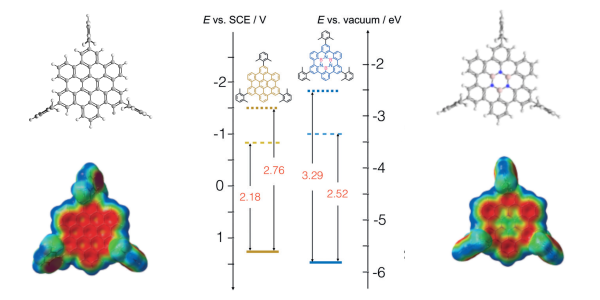
\includegraphics[width=\textwidth]{./images/dosso-combined}
	\caption{Electronic structure of HBC (left) and HBBNC (right). The even electrostatic potential (shown as colored models) for HBC is changed for HBBNC at the center where the molecule is doped with boron and nitrogen. This does deplete the electron density at the center. The electronic gap is calculated (center) and shows a smaller gap for HBC (\SI{2.18}{\eV}) compared to HBBNC (\SI{2.52}{\eV}). Adopted from \cite{dosso_synthesis_2017}}
	\label{fig:HBC+HBBNC-electronics}
\end{figure}

The present functionalization of the coronene molecule serves a twofold purpose. The functionalized core of the molecule is used to create 1. an sufficiently large adsorption platform for small polar molecules (like CO) and 2. an electrostatic potential surface to trap polar species. 
%Due to the different electro negativity of the atomic species in the center adsorption of gases in the central part can be interesting effects to look out for. 
Di-Methylphenyl groups are added to lift the molecule from the substrate and guide the formation of self-assembled islands of the molecule on the surface while electronic interactions with the substrate are reduced. Molecules are provided by the group of Prof.\ Dr.\ D.\ Bonifazi, Jacobo Dosso performed the synthetization of the molecules. 

\section{Results}
After RT adsorption of HBBNC on Ag(111) different assemblies are found. 
\begin{figure}[]\centering
	\subfigure[Hexamer self-Assembly after RT adsorption.]{
		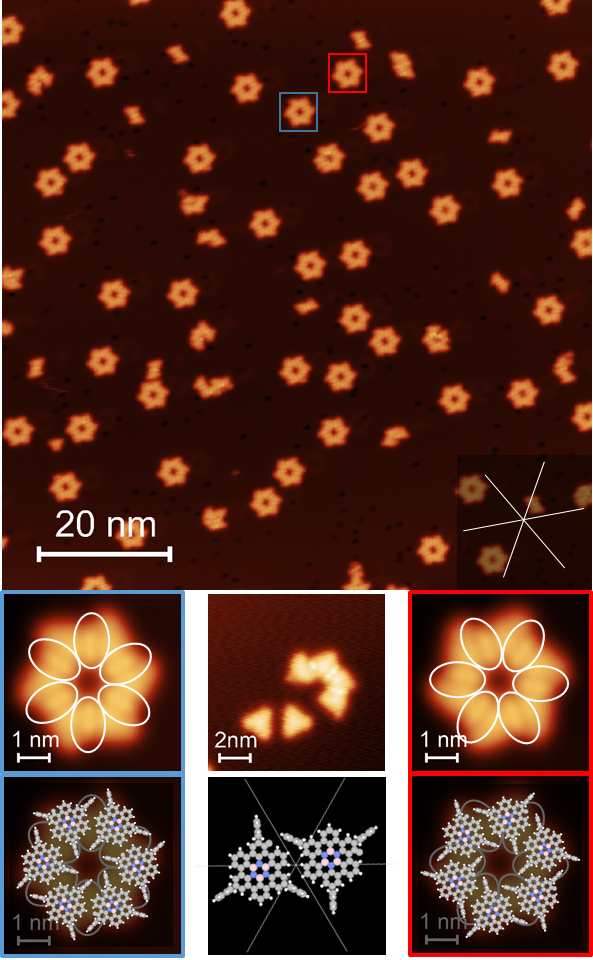
\includegraphics[height=0.7\textwidth]{./images/HBBNC-RT-assembly-2}
		\label{fig:HBBNC-low-coverage}
	} \quad
	\subfigure[Line spectrum for disassembled hexamer.]{
		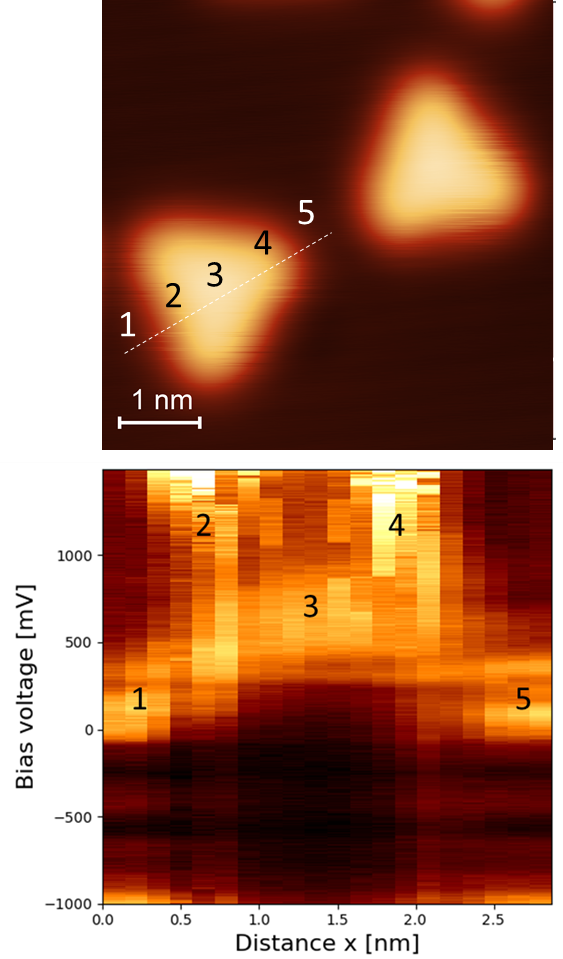
\includegraphics[height=0.7\textwidth]{./images/HBBNC-RT-spectra}
		\label{fig:HBBNC-spectra}
	}
	\caption{Low coverage RT adsorption of HBBNC on Ag(111). \subref{fig:HBBNC-low-coverage} Molecular self-assembly. An overview image is shown on top, where crystal orientation (white lines) and two hexamer orientations (red,blue) are shown. White ellipses highlight features in apparent height that do not appear for single molecules. In between, lateral disassembly of a single hexamer into single molecules is shown. Last line shows molecular models for each hexamer orientation. \subref{fig:HBBNC-spectra} STM topography (top) together with a set of spectra along the points indicated across the lower left molecule (bottom). Five points are highlighted by numbers. Bottom: dI/dV spectra for each point. Imaging parameter: \subref{fig:HBBNC-low-coverage} \SI{88.5}{\nano \meter}, \SI{750}{\milli \volt}, \SI{0.1}{\nano \ampere}, Color scale: \SIrange{0}{400}{\pico \meter}, \subref{fig:HBBNC-spectra} \SI{5.5}{\nano \meter}, \SI{750}{\milli \volt}, \SI{0.2}{\nano \ampere}, Color scale: \SIrange{0}{250}{\pico \meter}.}
	\label{fig:HBBNC-assembly-spectra}
\end{figure}
For low coverage (left side in \autoref{fig:HBBNC-assembly-spectra}) the dominating pattern is a hexagon in two different orientations (blue/red) with respect to the substrate.  Following things can be concluded: 

1. The internal structure of these hexamers can be revealed by lateral manipulation of a hexamer with the STM tip. A hexagon is made up of six intact HBBNC molecules. The monomer shape resembles a triangle with even apparent height distribution. A closer look on the modeled assembly of the hexamers shows two possible molecular orientations present for both hexamer types. The molecular orientation aligns along the high symmetry directions of the substrate. This is true for the few di- and trimer assemblies present, too. Two neighboring molecules are rotated by \SI{180}{\degree} and connect to each other with parallel edges, shifted to avoid steric hindrance. The center-center distance is \SI{1.5 \pm 0.1}{\nano \meter}. 

2. The two bright features in apparent height between two neighboring molecules (highlighted by white ellipses in \autoref{fig:HBBNC-assembly-spectra}) only occur when two molecules are close to each other and show the right inter-molecular orientation. Otherwise only a single or no protrusion at all is imaged. Therefor these features are attributed to rotated di-methyl-phenyl rings that resemble the shape of the gas-phase calculated structure. These protrusions are best visible at negative bias voltages, but are present for a wide range of positive and negative bias voltages. This is an indication for a true geometrical change and not an electronically induced feature in STM.

3. Molecules not incorporated in a hexamer appear flat with no pronounced apparent height features above the legs. This further benefits the assumption of flexible legs, that adjust their rotation to the surrounding. While arranging flat for monomers, the close proximity in assemblies causes a rotation. Because a leg orientation may be hard to access in STM (compare EHT simulation in \autoref{fig:HBBNC-EHT-leg-configuration}) further AFM measurements on the geometrical structure are done and show possible conformational changes in the molecule (\autoref{fig:HBBNC-nc-AFM-legs-change}).

Both types of hexamers are equally often present on the surface. From the observation of smaller hexamer fragments, it seems like the growth mechanism of the hexamers is already fixed in an early state of the assembly and depends on the adsorption site of the second molecule attaching to the first. Molecule by molecule than arranges to match the steric hindrance restrictions from the already formed parts of the hexamer. This efficient guiding mechanism leads to most molecules finish hexamer assemblies. Since only two possible arrangements for the first molecules are possible, two different hexamer configurations are found.

The electronic structure of single HBBNC molecules is investigated with STS after disassembly of a hexamer into its comprising single molecules. At the right side in \autoref{fig:HBBNC-assembly-spectra} two former hexamer constituents are shown in an STM topography image. A series of twenty STS spectra is taken along the dotted line and imaged below. Numbers indicate special positions for these spectra. 1 and 5 refer to positions on the silver substrate close to the molecule. 2,3,4 are taken at the edge, center and corner of the triangular molecular footprint. There is a pronounced electronic feature around 650 mV on the molecular center, features at \SI{1200}{\milli \volt} and \SI{1600}{\milli \volt} can be attributed to the leg and edge positions respectively. The lateral distribution of electronic features within the molecule is further evidenced by dI/dV maps recorded at the stated values (\autoref{fig:HBBNC-Ag111-dIdV-maps}).
The surface state of the substrate (\SI{-50}{\milli \volt} next to the molecule) vanishes below the molecule or shifts to positive bias values. At negative bias energies, faint tip states are visible that maintain their position in energy. 

%\begin{figure}[]\centering
%	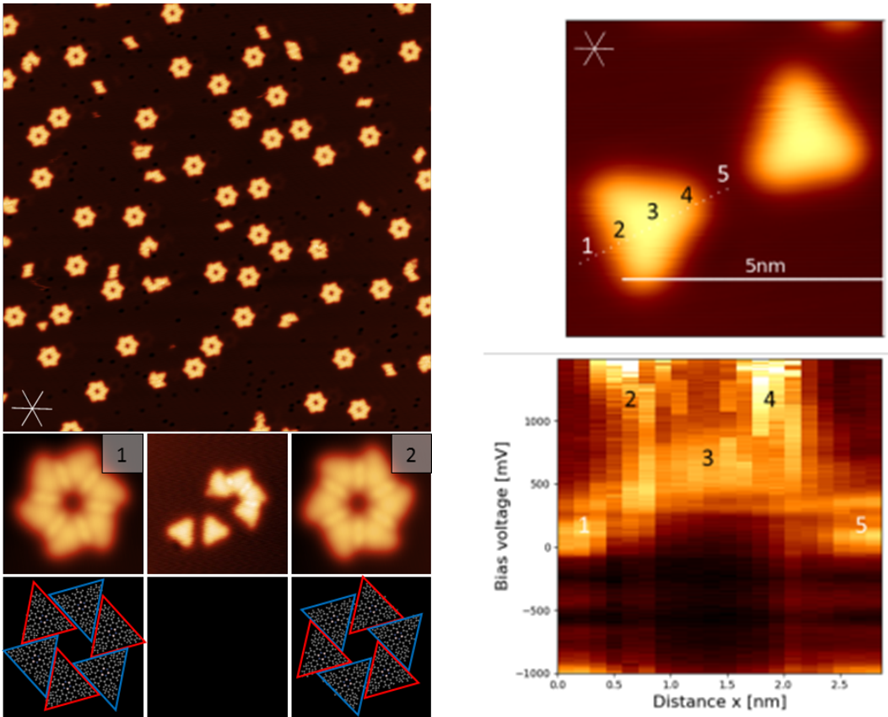
\includegraphics[width=\textwidth]{./images/test}
%	\caption{Low coverage assembly of HBBNC after RT adsorption on Ag(111). An overview image is shown on top, two hexamer orientations (1,2) are shown below. In between, lateral disassembly of e single hexamer into single molecules is shown. Last line shows molecular models for each hexamer orientation. \textcolor{red}{Imaging parameter: \SI{11.07}{\nano \meter}, \SI{1.5}{\volt}, \SI{0.1}{\nano \ampere}}. Top: STM topography: Set of spectra along the points indicated across the lower left molecule. Special points are indicated by numbers. Bottom: dI/dV spectra for each point, starting from one to five. \textcolor{red}{Renew scalebar, Imaging parameter: \SI{11.07}{\nano \meter}, \SI{1.5}{\volt}, \SI{0.1}{\nano \ampere}}.}
%	\label{fig:HBC+HBBNC-electronics}
%\end{figure}



%%%%%%%%%%%%%%%%%%%%%%%%%%%%%%%%%%%%%%%
% SINGLE WRAPFIGURES 
%\begin{wrapfigure}{R}{5cm}\centering
%	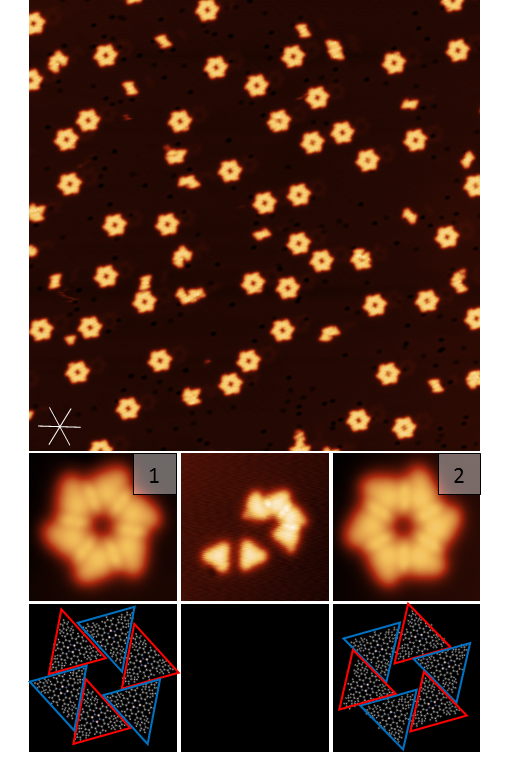
\includegraphics[width=5cm]{./images/hbbnc-ag-111-rt}
%	\caption{Low coverage assembly of HBBNC after RT adsorption on Ag(111). An overview image is shown on top, two hexamer orientations (1,2) are shown below. In between, lateral disassembly of e single hexamer into single molecules is shown. Last line shows molecular models for each hexamer orientation. \textcolor{red}{Imaging parameter: \SI{11.07}{\nano \meter}, \SI{1.5}{\volt}, \SI{0.1}{\nano \ampere}}.}
%	\label{}
%\end{wrapfigure}
%
%\begin{wrapfigure}{R}{5cm}\centering
%	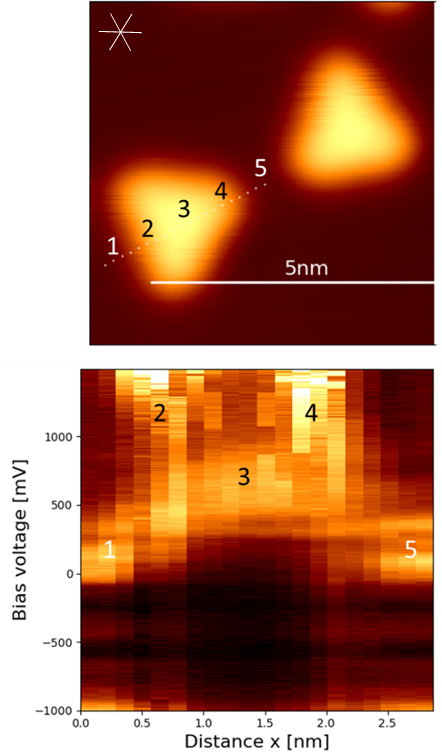
\includegraphics[width=5cm]{./images/hbbnc-ag-111-rt-linespectrum}
%	\caption{Top: STM topography: Set of spectra along the points indicated across the lower left molecule. Special points are indicated by numbers. Bottom: dI/dV spectra for each point, starting from one to five. \textcolor{red}{Renew scalebar, Imaging parameter: \SI{11.07}{\nano \meter}, \SI{1.5}{\volt}, \SI{0.1}{\nano \ampere}}.}
%	\label{}
%\end{wrapfigure}
%%%%%%%%%%%%%%%%%%%%%%%%%%%%%%%%%%%%%%%

Increasing the coverage leads to island formation with two dominant island types shown in \autoref{fig:HBBNC-med-coverage-2}. The first can be described as coalesced hexamer configuration. All of the hexamers within an islands show the same orientation and maintain their inner binding motif upon contact. The unit cell is rhombic with an opening angle of \SI{60}{\degree} and \SI{4.2 \pm 0.1}{\nano \meter} long legs. It holds six molecules and is rotated by \SI{30}{\degree} with respect to the subtrate's dense packed direction. The connection point between three hexamers shows almost every time a bright feature in STM. Since here no molecular entities reside, this is attributed to another adsorbate. 

The second island type is made of chain motifs which did not show up on lower coverage. These chains consist of molecules in two orientations which were already present for the hexamer configuration. Opposed to the latter, the second type is made of two chain orientations with varying length, so that little long range order is achieved. \autoref{fig:HBBNC-med-coverage-2} shows such an island together with two hexamers. The molecular model shows two parallel chains as they guide the island formation. These two are separated by $\approx \SI{6}{\nano \meter}$. The clearance is filled by repeating sets of four molecules acting as connection segment between chains. The inner pair of this connection shows the same binding configuration as the chain motif, but is rotated by \SI{30}{\degree}. Two additional molecules connect those two to the chains. Their orientation is close to the molecules' constituting the chains. The close proximity of the molecules between the chains however results in the deformation of the leg functionalization and additional apparent height features in STM. Although flexible side groups allow for a denser packing, without which the molecules would not fit in the space between two chains, it hampers the exact determination of the molecular assembly. The notable change to the gas phase configuration can be seen in the overcrowded region for the gas phase modeled assembly shown in the image. The unit cell however is $(\SI{5.9 \pm 0.1}{} \times \SI{2.9 \pm 0.1}{})\SI{}{\nano \meter \squared}$ large, with an angle of \SI{70}{\degree} betweenits legs. It holds five molecules and its long side is close to the crystal substrate's high symmetry direction, with a mismatch of $\leq \SI{5}{\degree}$. The chain length is always a multiple of 2 molecules and often shorter than eight molecules.  At rare occasions, a square pattern is formed which is shown in \autoref{fig:HBBNC-medium-coverage-different-motifs}.

\begin{figure}[] \centering
	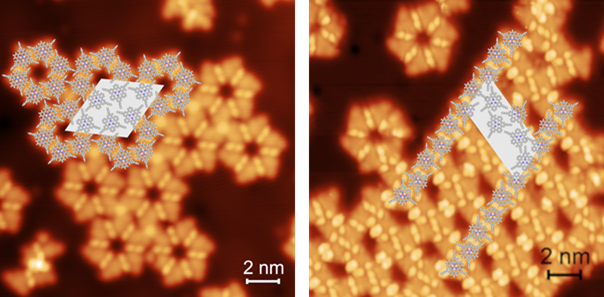
\includegraphics[width=\textwidth]{./images/hbbnc-ag-111-rt-med-coverage-2}
	\caption{Medium coverage adsorption of HBBNC at RT on Ag(111). While the hexagons are still present, regular assemblies with coalesced hexamers and chains occur. Imaging parameter: \SI{20}{\nano \meter}, \SI{-250}{\milli \volt}, \SI{0.2}{\nano \ampere}.}
	\label{fig:HBBNC-med-coverage-2}
\end{figure}

Further increasing the coverage results in dense regions being formed (shown in \autoref{fig:HBBNC-high-coverage}). The dense packing results in a complex pattern of rotated side groups.

To address questions of thermal stability of the assembly and the molecule itself, annealing experiments are performed. A sample prepared at RT has been annealed in vacuum to \SI{350}{\celsius} and \SI{420}{\celsius} and is investigated with the STM (\autoref{fig:HBBNC-annealing}).

After the sample is annealed to \SI{350}{\celsius} only monomers and few random agglomerates remain on the surface. Although the molecules undergo the same temperature range where hexamers are formed (from RT to \SI{5}{\kelvin}) no regular assembly is imaged. Because the assembly is guided by the presence of the dimethylphenyl group a closer look to the molecular conformation is taken. Three different types can be distinguished and are shown in the inset. 
1: The abundant species are molecules with a single protrusion on the leg position.
2: Flat molecules with an even apparent height at the legs are present, but are a minority.
3: Molecules with a leg missing are rarer exceptions.
The unstable imaging conditions above some of the molecules legs indicate their flexibility while the others seem to be rigidly connected to the molecular backbone and therefor imaged stable. The vanishing hexagon binding motif - observed for the RT prepared sample - underpins the importance for the molecules leg to adopt the assembly. This flexibility is not present any more after annealing to \SI{350}{\celsius} and hexamer formation is suppressed.
%\textcolor{red}{\textbf{Molecular orientation?}}

Increasing the annealing temperature to \SI{420}{\celsius} results in a percolated network where monomers  coalesce and connect via their legs. Lateral manipulation attempts indicate a connection between neighboring molecules. Opposing to the previous preparations, the assembly could not be divided into single monomers. This rigid connection indicates a covalent coupling of the molecules. 
%\textcolor{red}{\textbf{Molecular orientation?}}


\begin{figure}[h!]\centering
	\subfigure[Annealing to \SI{350}{\celsius}]{
		\includegraphics[width=0.45\textwidth]{./images/hbbnc-annealing-a}
		\label{fig:HBBNC-annealing-350}
	} \quad
	\subfigure[Annealing to \SI{420}{\celsius}]{
		\includegraphics[width=0.45\textwidth]{./images/hbbnc-annealing-b}
		\label{fig:HBBNC-annealing-420}
	}
\caption{Annealing steps of HBBNC on Ag(111) after RT adsorption. \subref{fig:HBBNC-annealing-350} After annealing to \SI{350}{\celsius} and cooling down to LT-STM temperatures no hexamers are visible. A variety of molecular orientations and different conformations are present (inset). \subref{fig:HBBNC-annealing-420} Annealing the same sample to \SI{420}{\celsius} leads to an unregular network where molecules are connected via their legs and not separable by lateral manipulation. Imaging parameter: \subref{fig:HBBNC-annealing-350} Width: \SI{40}{\nano \meter}, \SI{750}{\milli \volt}, \SI{0.1}{\nano \ampere}, Inset \SI{10}{\nano \meter}, \SI{500}{\milli \volt}, \SI{0.1}{\nano \ampere}. \subref{fig:HBBNC-annealing-420} Width: \SI{40}{\nano \meter}, \SI{2}{\volt}, \SI{0.1}{\nano \ampere}, Inset \SI{10}{\nano \meter}, \SI{2}{\volt}, \SI{0.5}{\nano \ampere}}
\label{fig:HBBNC-annealing}
\end{figure}

%
%\begin{figure}[] \centering
%	\includegraphics[width=0.7\textwidth]{./images/hbbnc-annealing}
%	\caption{Annealing steps of HBBNC on Ag(111) after RT adsorption. Left: After annealing to \SI{350}{\celsius} and cooling down to LT-STM temperatures no hexamers are visible. A variety of molecular orientations and different conformations are present (inset). Right: Annealing the same sample to \SI{420}{\celsius} leads to an unregular network where molecules are connected via their legs and not separable by lateral manipulation. 350°C: Imaging parameter: Width: \SI{40}{\nano \meter}, \SI{750}{\milli \volt}, \SI{0.1}{\nano \ampere}, inset \SI{10}{\nano \meter}, \SI{500}{\milli \volt}, \SI{0.1}{\nano \ampere}. 420°C: Imaging parameter: Width: \SI{40}{\nano \meter}, \SI{2}{\volt}, \SI{0.1}{\nano \ampere}, inset \SI{10}{\nano \meter}, \SI{2}{\milli \volt}, \SI{0.5}{\nano \ampere}}
%	\label{fig:HBBNC-annealing}
%\end{figure}

Since the formation of a new bond is expected to change the core levels of participating elements (Carbon, C\textit{1s}), XPS measurements at the NIM-XPS are done and presented in the following. Sub-ML as well as multilayer preparations have been annealed to \SI{420}{\celsius} to quantify a possible change in binding energy. 

After RT deposition of a sub-ML HBBNC on Ag(111) a C\textit{1s} peak is observed at $\SI{284,94 \pm 0.01}{\eV}$ that grows with increasing coverage and gradually shits to $\SI{285,43 \pm 0.01}{\eV}$. There is a minor shift after adsorption of a multilayer, because molecules in the second layer are facing a different environment.
After annealing of the multilayer preparation the C\textit{1s} peak shifts to lower binding energies ($\SI{284,59 \pm 0.01}{\eV}$), below the value observed for sub-ML preparation. A behavior typical for cyclodehydrogenation and ring closure reactions of e.g. porphyrins \textcolor{red}{(\textbf{citation})}.

\textcolor{red}{Other mechanisms for a shift towards lower binding energies include the transfer of negative charge into the molecule. The more electrons agglomerated the better the atomic core charge is screened from the C\textit{1s} electrons. As a result the charge "felt" by electrons decreases and their binding energies with it. 
	The opposite effect occurs for elements that strongly  withdraw charge from carbon (like fluorine, chlorine), and is less present for elements like nitrogen and oxygen that only slightly shift the binding energy towards positive values.
As the molecule becomes flat, it interacts more with the substrate surface. It is likely that the electron $\pi$ system of the carbon rings interacts most with the substrate, due to its geometry exceeding the molecule and possible penetrating the substrate. To lower the binding energies for the carbon species, charge needs to be transferred from the substrate into the molecule.
	This would also imply less interaction with the metallic substrate for the multilayer preparations and an corresponding shift in the C\textit{1s} peak towards higher binding energies. 
It is assumed that the C-H bonds in the perimeter of the molecule are more reactive than the carbons bound to other carbons only and thus contribute more to the charge substitution with the substrate. \cite{medeiros_benzene_2012}}

The area below the peak drops to a sub-ML coverage, a clear indication for desorption of the multilayer. A covalently coupled layer would not desorp, so coupling in the lowest layer takes place after multilayer desorption.
It can be concluded that annealing HBBNC on a Ag(111) surface will lead to the formation of a network stabilized via interactions that involve carbon 

\begin{figure}[] \centering
	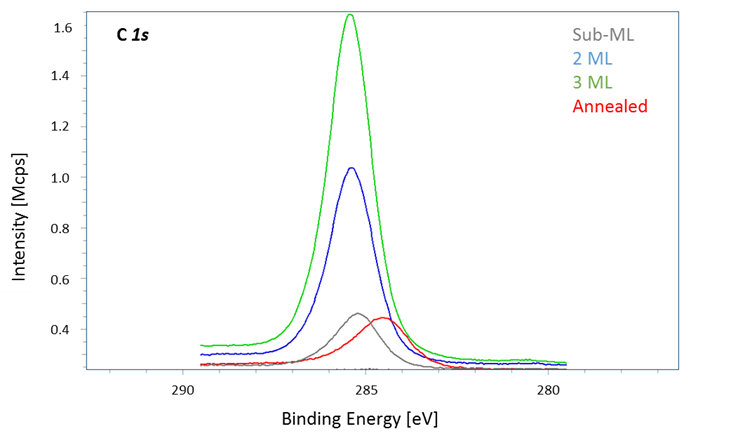
\includegraphics[width=0.7\textwidth]{./images/hbbnc-xps1}
	\caption{XPS C\textit{1s} spectra of HBBNC adsorbed at RT on Ag(111) for increasing coverages. Annealing to \SI{420}{\celsius} leads to a decrease in signal and shift to lower binding energies.}
	\label{}
\end{figure}

To further check the conformational changes in the molecule due to annealing, AFM measurements are done. nc-AFM has the big advantage over STM that it is less sensible to electronic changes in the molecule – more closely resembling the true geometric shape.

\textbf{Before annealing} 
HEXAMER COnFIguraTIoN in AFM

\textbf{After annealing}
The fused triangular molecules that appeared flat in STM after annealing to \SI{420}{\celsius} reveal their interesting geometric properties when investigated by means of nc-AFM. It is observed that many of the molecules appear to have their dimethylphenyl groups aligned planar to the surface. A behavior expected for a ring closure reaction between the hexabenzol groups and dimethylphenyl legs.

In the present case, almost all molecules show some defined contrast in the connection region which is an indication for a chemical interaction between the molecules.
\autoref{fig:HBBNC-linking} shows a dimer configuration that is used to clarify the structure of this connection with sub molecular resolution. For the two molecules a center-center distance can be measured (\SI{1.8 \pm 0.1}{\nano \meter}) and is used as benchmark for model verification. The detailed AFM image emphasizes that a link between molecules is present i) either between a leg functionalization and the coronene body (Type I: \autoref{fig:HBBNC-link-lost-groups-AM1}) or ii) between legs (Type II: \autoref{fig:HBBNC-link-lost-hydrogen-AM1}). For both configurations the center-center distances are derived from the AM1 optimized models and result in a closer arrangement for type I (\SI{1.45 \pm 0.01}{\nano \meter}) as for type II (\SI{1.72 \pm 0.01}{\nano \meter}). A close match between the center-center distance of type II and the experimental value ($\delta \leq \SI{6}{\percent}$) is achieved.

Both connection types increase the number of carbon rings and thus result in additional features visible in AFM. For type I the close link between leg and molecular core makes up for four new rings being formed, while a connection solely via the legs creates only one additional ring. This becomes most apparent in the planar configuration of both types (\autoref{fig:HBBNC-ring-structure}). This is not discussed in detail however, since the contrast in AFM is subject to changes in tip functionalization and scan height.

\begin{figure}[] \centering
	\subfigure[Raw AFM image of HBBNC on Ag(111) after annealing to \SI{420}{\celsius}. The distance between the two righmost molecules that form a dimer is \SI{1.8 \pm 0.1}{\nano \meter}]{
		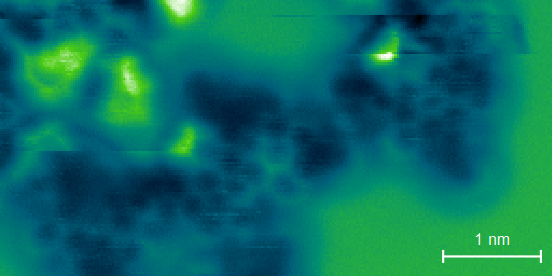
\includegraphics[width=0.7\textwidth]{./images/00337_180608-freq}
		\label{fig:HBBNC-link-AFM-freq}
	}
	\subfigure[Simulated AFM image for type I. Molecular centers are \SI{1.45 \pm 0.01}{\nano \meter} apart.]{
		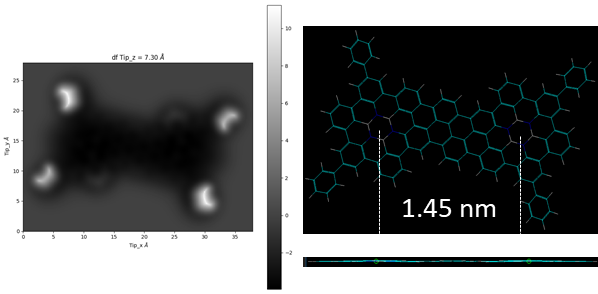
\includegraphics[width=0.35\textwidth]{./images/00337-missing-methyl-group-link-2-AM1-model}
		\label{fig:HBBNC-link-lost-groups-AM1}
	} \quad
	\subfigure[Simulated AFM image for type II. Center-center distance increases to \SI{1.72 \pm 0.01}{\nano \meter}.]{
		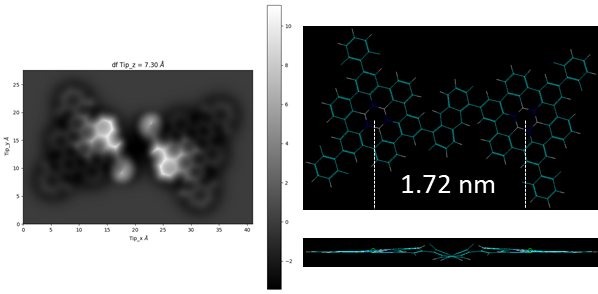
\includegraphics[width=0.35\textwidth]{./images/00337-AM1-methyl-groups-fuse-link-2-split-hydrogen}
		\label{fig:HBBNC-link-lost-hydrogen-AM1}
	}
	\subfigure[Connection type I but with planar molecules (no AM1 optimization). Slightly smaller molecule distance of \SI{1.70 \pm 0.01}{\nano \meter}]{
		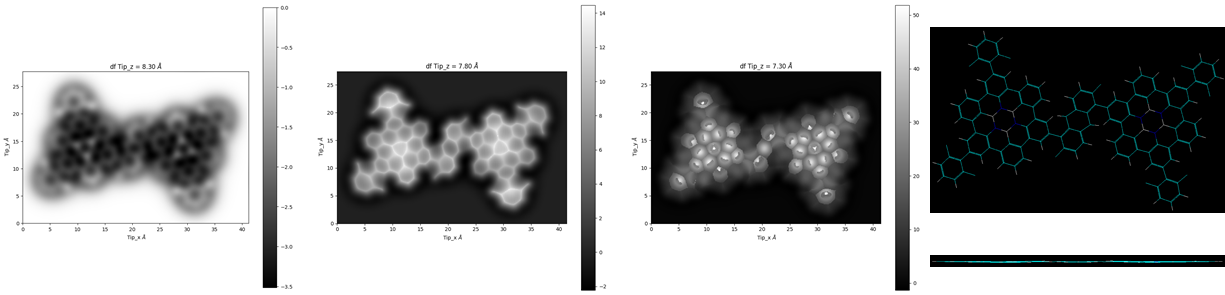
\includegraphics[width=0.7\textwidth]{./images/00337-methyl-groups-fuse-link-2-split-hydrogen-detail}
		\label{fig:HBBNC-link-lost-hydrogen-guess}
	}
	\caption{Structure of a intermolecular connection between HBBNC on Ag(111) after annealing to \SI{420}{\celsius}. AFM image \subref{fig:HBBNC-link-AFM-freq} together with simulated AFM images of two different binding motifs. \subref{fig:HBBNC-link-lost-groups-AM1} Linking between leg and coronene center. This link may occur after the dimethyl groups at the phenyl legs are cleaved. \subref{fig:HBBNC-link-lost-hydrogen-AM1} Covalent bond formation after dehydrogenation of di-methyl-functions. The bond is formed via the remaining carbon of the methyl group and and adjacent phenyl ring and is present twice for each link. A slight ripple present close to the covalent bond is a result from the AM1 structure optimization performed. \subref{fig:HBBNC-link-lost-hydrogen-guess} shows the same bond motif as \subref{fig:HBBNC-link-lost-hydrogen-AM1} but for planar geometries and three different scan heights. The binding distances compare best for a bond via legs (configurations \subref{fig:HBBNC-link-lost-hydrogen-AM1} and \subref{fig:HBBNC-link-lost-hydrogen-guess}) with a mismatch of $\leq \SI{6}{\percent}$.}
	\label{fig:HBBNC-linking}
\end{figure}

%\begin{figure}[] \centering
%	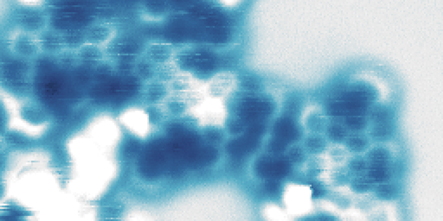
\includegraphics[width=0.7\textwidth]{./images/hbbnc-annealed-afm}
%	\caption{AFM image displaying the Laplace filtered frequency shift channel. While rings constituting the molecule are visible, features in between rigid molecular connection are visible. \textcolor{red}{Scalebar, Imaging parameter: \SI{11.07}{\nano \meter}, \SI{1.5}{\volt}, \SI{0.1}{\nano \ampere}}.}
%	\label{}
%\end{figure}

\textbf{Accounting for variing number of visible rings}
Through assignment of geometric shape and features in AFM images a good agreement between molecular model and image can be achieved and helps to clarify the bond motif between molecules. This relies on the number and position of imaged carbon rings and fixes the resulting bond distances. 
 Due to some flexibility of the leg functionalization the bond angle and distance may vary. In the following the influence of changing molecular geometry during the annealing process is discussed briefly.
 
The annealing temperature not only assists the covalent bond formation between legs, but may result in a intramolecular bond being formed. Hereby the leg functionalization rotates in plane and reduces the distance to the coronene backbone, a bond between methyl group and coronene carbon ring may result in the formation of a 5-membered ring as shown in \autoref{fig:HBBNC-ring-closure}. Depending on the turn direction, two different leg orientations are possible, kinked to whichever rotation direction was chosen.

When these species now engage each other with the same bond motif as derived earlier, different bond geometries result. \autoref{fig:HBBNC-ring-closure-motifs} shows the same type of bond for pristine HBBNC molecules  \subref{fig:HBBNC-AM1-methyl-groups-fuse-link-2-split hydrogen} and its ring-closed complement \subref{fig:HBBNC-Closed-ring-dimer-1}. These differ in shape of the intermolecular connection and the number of carbon ring structures within the dimer. This change however is hard to measure in AFM since geometric configuration after adsorption on a metal is hardly emphasized by present calculations and influences the appearance.

Since a ring closure fixes the leg orientation the resulting dimer shows a fixed orientation of its constituents which are modeled here either parallel or rotated by \SI{180}{\degree} with respect to each other.

A preparation where RT adsorped molecules are annealed to \SI{420}{\celsius}, cooled down to RT is prepared and HBBNC is evaporated at RT afterwards. See \autoref{fig:HBBNC-anneal-RT} for details. It shows the two binding motifs that were observed for the annealed sample (covalently fused molecules in unregular structures) and for adsorption at RT (formation of hexamers). No mixed structures are observed, hardening the assumption that HBBNC form covalent bonds and the resulting network does not allow for connection to pristine HBBNC.

\textbf{On Au(111)}To have the molecule adsorbed flat on the surface, another substrate is chosen. Silver is known to have a larger impact on adsorption geometries than Au(111) has.

In contrast to adsorption on Ag(111) where almost all molecules are incorporated into hexamers, molecules separate into monomers after RT adsorption on Au(111). Molecules arrange in the herringbone reconstruction visible as bright stripes in the STM image. These divide the surface into regions of fcc and hcp reconstruction.

Molecules show two different appearances. While some appear to adsorb flat in STM, others already show a protrusion above one of their legs. This protrusion is not caused by parts of the herringbone reconstruction, as two molecules on very similar adsorption sites within the reconstruction show different appearances.

\begin{figure}[] \centering
	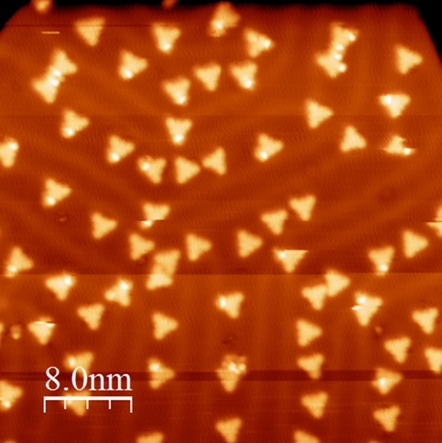
\includegraphics[width=0.5\textwidth]{./images/hbbnc-au-111-rt}
	\caption{STM topography image of HBBNC on Au(111)/Mica. \textcolor{red}{\textbf{Stripes}} of the herringbone reconstruction divide the surface into regions of fcc and hcp stacking order. Only monomers form after adsorption at RT. \textcolor{red}{Scalebar, Imaging parameter: \SI{11.07}{\nano \meter}, \SI{1.5}{\volt}, \SI{0.1}{\nano \ampere}}.}
	\label{}
\end{figure}

The adsorption geometry of monomers is investigated. By scanning the same molecule in different heights, elevated parts of the molecule can be easily distinguished by their larger interaction force with the tip (the involved larger frequency shift is shown as protrusion in nc-AFM images). These show that the dimethylphenyl legs of a monomer do not lie flat on the surface but have an elevated and lower lying part. While their initial orientation on the surface is likely determined at adsorption, the legs are able to flip under the influence of the AFM tip (see \autoref{fig:HBBNC-nc-AFM-legs-change-calc}) and change the adsorption angle of the molecule. This is imaged as bright edge where the lower part of the rotated dimethylphenyl group lifts the molecule. The effect is most pronounced when neighboring groups rotate in opposite directions. This is underpinned by calculated AFM images (\autoref{fig:HBBNC-nc-AFM-legs-change}) that show the same feature pattern after gentle rotation of the side groups. 

\section{Summary \& Discussion}
%It is reported that for hexa-peri-benzocoronene, no stable second layer of molecules can be found for a strong electron donor like HBC at solid-solution interface\cite{de_feyter_two-dimensional_2003}.
Investigations with STM are performed for similar molecules on Au(111) by \cite{Krieg_construction_2015}.

HBBNC has been deposited at RT on Ag(111) and Au(111). On Ag(111) different assemblies are formed depending on coverage. Although the molecule is not chiral in gas phase, low coverage adsorption on the Ag(111) surface leads to the formation of hexagon assemblies with corresponding mirror images. During adsorption the molecule rotates its legs to a more planar configuration with the substrate. 

This compares to previous studies of coronene on Ag(111), where close packed assemblies were formed at a distance of \SI{1.15}{\nano \meter} which is of course smaller due to the smaller molecule.\cite{lackinger_coronene_2002} Hexa-peri-hexabenzocoronene assembles in close packed hexagonal structure on HOPG with $a =\SI{1,37}{\nano \meter}$.\cite{samori_epitaxial_2002}

The close resemblence of HBCs assembly suggests that the orientation of single molecules with respect to the substrate is given by the symmetry of the molecule alone and that HBBNC's BN core does not influence the adsorption compared to the carbon center of HBC. These findings compare well with previous results. Coronene was investigated with STM on Ag(111) \cite{lackinger_coronene_2002, mckinnon_observation_1995}. Together with hexa-peri-benzocoronene its orientation at sub-ML regimes is determined by the molecular symmetry matching the substrate high symmetry directions\cite{zimmermann_epitaxial_1992}.

Although tried intensely, the calculated band gap of \SI{2.52}{\eV} is not observed and may point to a broad HOMO feature that blends with the often observed tip states.
Charge transfer between molecule and metallic substrate is possible and may be evidenced by future calculations.

Increasing the coverage in the high sub-ML regime leads to island formation with different unit cells. The interaction between molecules is always guided by the orientation of the di-methyl functional groups and results in chains formation.

Interestingly, exceeding monolayer coverage lead to stable second layer formation only for the HBBNC species, while no second layer is observed at RT adsorption of HBC on Ag(111), although multilayer coverage of hexa-peri-benzocoronene is reported and believed to change the adsorption geometry to a tilted configuration\cite{zimmermann_epitaxial_1992} where increasing molecular $\pi-\pi$ interactions between molecular planes cause a \SI{0,3}{\eV} shift of the molecular levels toward higher binding energy\cite{glowatzki_hexa-_2008}.

Annealing a multilayer HBBNC preparation to \SI{420}{\celsius} leads to a chemical coupling between molecules that is pointed at by combined STM, XPS and AFM measurements. 
